
\begin{figure*}[!tbp]
    \centering
    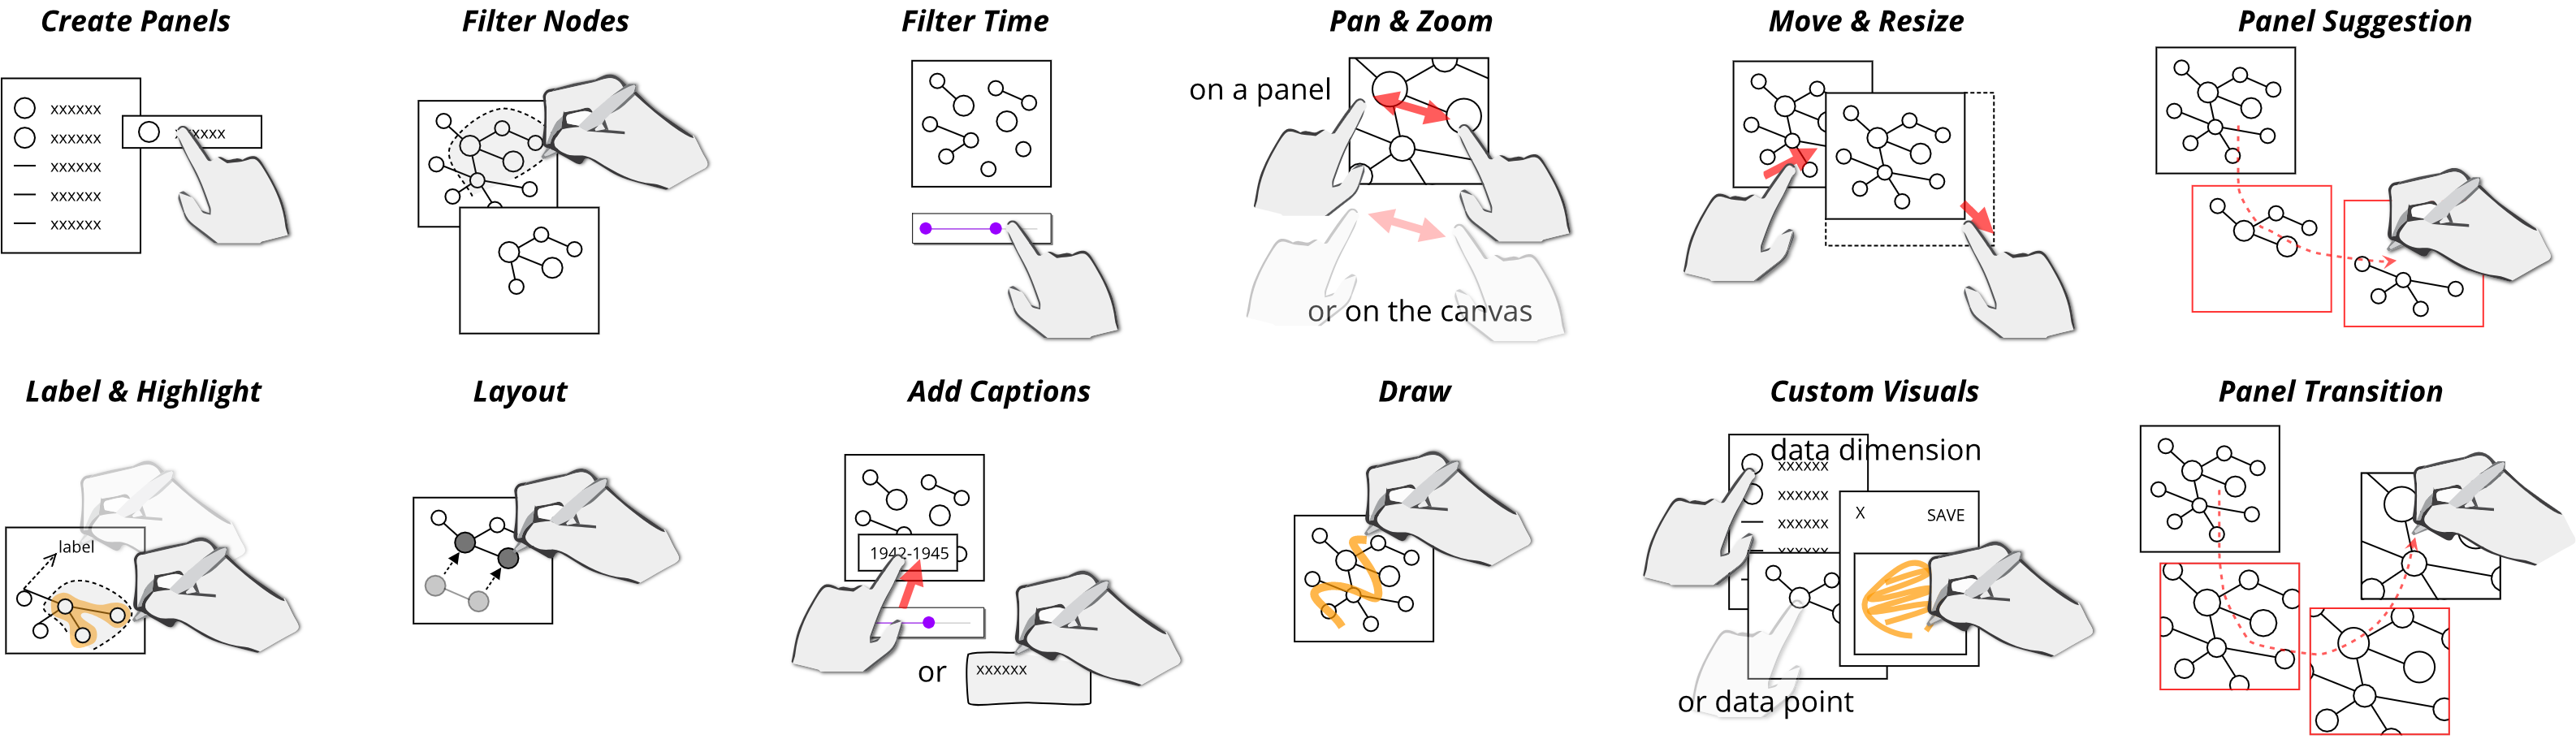
\includegraphics[width=1.0\textwidth]{figures/interaction.png} 
    % \vspace{-0.4cm}
    \caption{An overview of the pen + touch interactions supported by \toolname{}.}
	\label{fig:interaction}
    % \vspace{-0.4cm}
\end{figure*}

\section{\toolname{}}
\label{sec:datatoon}

We designed \toolname{} for a broad range of people who wish to craft data comics that communicate insights about their data. This may include graphic designers without programming expertise, data analysts without design expertise tasked with communicating their findings, or educators seeking new ways to engage their students. %\matt{trying to relate this to our scenario and study participants}
% This sections describes \toolname{}'s interface and its pen + touch interactions. %\matt{section feels too long, too user-manual-esque}

\subsection{Data Abstraction}
%\matt{Promoting this paragraph based on R3's comments, though I haven't commented on network size limitations}
As mentioned in the introduction, we chose to focus on dynamic network data since it is poorly supported by existing communicative visualization and storytelling tools, and because of its inherent parallel to the dynamic interactions between characters appearing in comics.   
In particular, \toolname{} supports multivariate dynamic network data, which consists of nodes and links and their attributes. A node can have a label and a type, as well start and end dates. A link must have source and target nodes and may have a direction and a weight along with same set of attributes describing nodes. Given this criteria, \toolname{} also supports static networks, where neither nodes nor links have associated start or end times. Note that \toolname{} is primarily a storytelling tool, one suitable for communicating different aspects of dynamic network data; we do not address scalability issues and analysis tasks related to very large networks in this paper. 
  
\subsection{Story Abstraction}

Like a comic book, a data comic consists of pages (\autoref{fig:comicbook}), in which each page can contain multiple panels. A panel is the essential building block of a narrative structure, which can in turn contain visualization, images, text captions, and annotation.
% The relationship between panels is defined by their spatial positions that are often further complicated through varying sizes of the panels. 
The spatial arrangement of panels having varying size and content generates a unique narrative flow, enabling a nonlinear reading experience unlike linear sequences produced by other storytelling tools. 
% \matt{reuse the following later?}
% DataToon uses a comic book metaphor, allowing the author to create multi-page comics . Each page can embed a separate dataset, if necessary, to show a different facet of the story.
% The author can export each page into an image for printing and sharing. 
% Data filters, including type, temporal and node filters, and view transforms control the content of the panels, namely visualizations; that is, the underlying data is shared and reused across the panels so as mappings for custom visuals. Narration to highlight important aspects of the data or to convey data-driven messages is accomplished through the annotations. 

% A visual data story much relies on the elements of comics, integrated with data-driven abstractions. The model mainly consists of multiple panels, visualizations within the panels, and data-driven, visual and textual annotations. Panels are building blocks of a narrative structure. 

% focused tool set, data binding, rapid prototyping

% To allow people to craft expressive data representations (C1) as well as experiment with panel layout composition (C4), we opted to design \toolname{} as a pen+touch application. We reasoned that sketching afforded by the pen would stimulate creative and expressive designs, while direct touch interactions would encourage authors to experiment with panel arrangements.
%data comics via bimanual direct manipulation pen and touch interactions, overcoming the challenges described in \autoref{sec:data_comics}. 

\subsection{Interaction Design}

% The \toolname{} interface offers a focused set of instruments (materialized by different modes of use of the pen) to enable the creation, editing and styling of multiple panels representing different aspects of the data and experiment with their organization in space (materialized by a set of manipulable views on a zoomable canvas). 
\toolname{} is comprised of a canvas for storyboarding; content and legend panels for presenting visual representations of data; a set of pen tools for content creation and manipulation; and a contextual canvas for sketching custom visuals.

%that are contextually relevant to the elements of a data comic, from panels and pages to visualizations and annotations.
% A key aspect of \toolname{}'s design is to support data binding across panels, enabling functionality that other applications do not support, such as automatically propagating changes of visual representations to other panels to maintain consistency (C2) and automatically generating transitions between two panels (C3). % that have no connection to the underlying data.
% By combining a focused tool set with data binding, \toolname{} allows for rapid iterative design of data comics that could only be achieved via laborious manual efforts today.

% \subsection{User Interface}
% \toolname{} has a few main user interface components (\autoref{fig:tool_overview}). The page canvas (\autoref{fig:tool_overview}d) provides an authoring environment for managing visualization panels and drawing freeform annotations. The legend panel (\autoref{fig:tool_overview}d, upper left) not only shows the overview of visual mappings but also serves as an interface for creating content. The contextual canvas (\autoref{fig:workflow}i,j) is invoked on demand from the legend for customizing visual mappings, e.g., for sketching custom icons for nodes. The pen tool menu (\autoref{fig:tool_overview}a) allows the author to switch between functions from sketching to annotation and transition.
  
  
\autoref{fig:interaction} summarizes our pen + touch interactions. In general, our interaction design choices reflect the mantra: \textit{the pen writes, touch manipulates}~\cite{hinckley2010pen}. However, since individual nodes and links within panels are often too small to manipulate with a finger, the pen is also used to manipulate visual elements in some circumstances, as described below.  Throughout the interface, we chose to visually expose interactive controls rather than rely on implicit multi-touch gestures that are difficult to discover and remember. Note that we describe our final system, which improves upon the version used in our reproduction study described below.

% \matt{redundant}
% where touch always manipulates panels such moving and resizing). By default, the pen writes (
\includegraphics[scale=0.025]{figures/draw_pen.png}) but acquires different tools depending on the selected pen type (
\includegraphics[scale=0.025]{figures/label_pen.png} 
\includegraphics[scale=0.025]{figures/highlight_pen.png} 
\includegraphics[scale=0.025]{figures/filter_pen.png}  
\includegraphics[scale=0.025]{figures/magic_pen.png}  
\includegraphics[scale=0.025]{figures/layout_pen.png}). 


% In addition, visualization usually consists of a multitude of data points, making it cumbersome to manipulate using fingers.


% We made this design decision because a visualization usually consists of a multitude of data points, making it cumbersome to manipulate using fingers.

% It is cumbersome to manipulate the content mostly consisting of a fine-grained elements of a visualization. Thus, we decided to use the pen, instead of fingers, as a primary mode of interaction for the panel content. The pen acquires different functions depending on the pen type.  The pen eraser deletes the type of visual elements created through the pen type. 

% a list of node types and link types in the dataset. The pen tool menu allow users to acquire different pen functions applied to panels. A side menu for additional features such as undoing and redoing changes and importing the page to an external image file. (png and svg). 

\vspace{2mm}
\bpstart{Interacting with the canvas} 
\toolname{} provides an infinite canvas to support flexible authoring and rapid ideation, transitioning from data exploration to authoring activities (D3). The author can navigate the canvas via pan and zoom gestures. Meanwhile, using the pen, the author can draw or write anywhere on the canvas, either to annotate content or to add storyboarding notes and ideas. The author can create an empty panel by simply drawing a rectangle, to be filled later with content, or create panels from data. Panels can be freely arranged and resized with touch interactions, leading to different layouts at any point in the authoring process. 

%Our design decision for providing a flexible authoring environment is to allow for multiple workflows and fluidity in the iterative design process, while sketching can further amplify the expressive capability of such an environment due to its inherent informality % freeform and effortless nature
% \cite{xia2018dataink}.
\vspace{2mm}
\bpstart{Interacting with the legend panel}
A legend panel is created when the author drags a dataset file onto the canvas. This panel provides an overview of the dynamic network, displaying a list of node types and link types along with the cardinality of each type. 
%It plays a vital role in helping readers understand the visual encodings to the underlying data. 
%The author can import a dataset by dragging a data file onto the canvas (\autoref{fig:workflow}a). It causes a legend panel to appear, providing an overview of the dataset
This legend also serves as an interface for creating content panels. Dragging a node or link type from the legend onto the canvas creates a new content panel displaying a filtered visualization of the data. Dragging a node type automatically creates a unit chart of all nodes in the data matching this type. Dragging a link type automatically creates a force-directed node-link diagram of nodes connected by this link type. Note that links can convey both weight and direction via line thickness and arrows, should these optional attributes be provided. 

Node and link types can also be dragged from the legend panel to an existing content panel, whereupon its contents are updated to reflect the additional type (\autoref{fig:interface}E) and its layout recomputed. For instance, dragging a link type to a content panel containing a unit chart will convert the chart into a node-link diagram. Similarly, adding a link type to a panel containing a node-link diagram will generate multiple link types (see Figure~\ref{fig:interface}). 
% The core content of the panel is a visualization created from the legend panel. The number of data dimensions added to the panel determines the type and complexity of the visualization within. For example, multiple node types create a stacked unit chart , while having at least one link type generates a node-link diagram. Each node and link can use its shape size and line thickness respectively to encode a weight, while the link can additionally encode its direction (i.e., a simplified multivariate network). 
% The latter action is akin to adding a data filter to the panel. 
\vspace{2mm}

\bpstart{Interacting with content panels}
A content panel may contain visualizations, text, annotations, a background image, or some combination thereof (D1). Panels can  be nested: drawing a rectangle inside a panel creates a child panel, which is useful for text captions or inset visualizations. 
It is possible to duplicate an existing panel, copying all of the content of the source panel to a new panel (\autoref{fig:interface}I). This interaction is particularly useful for progressively building a narrative using the previous panel as a starting point.

Tapping on a panel containing a visualization selects it and enables panning and zooming within the panel. This also reveals a time slider for the panel, which applies additional temporal filtering to nodes and links displayed within the panel. Dragging this slider onto the panel creates a nested time caption panel (D2), which remains updates as the user changes the time slider (\autoref{fig:interface}K). 

%\matt{I forgot about this interaction. It doesn't seem very discoverable} 

\begin{figure}[b]
    \centering
    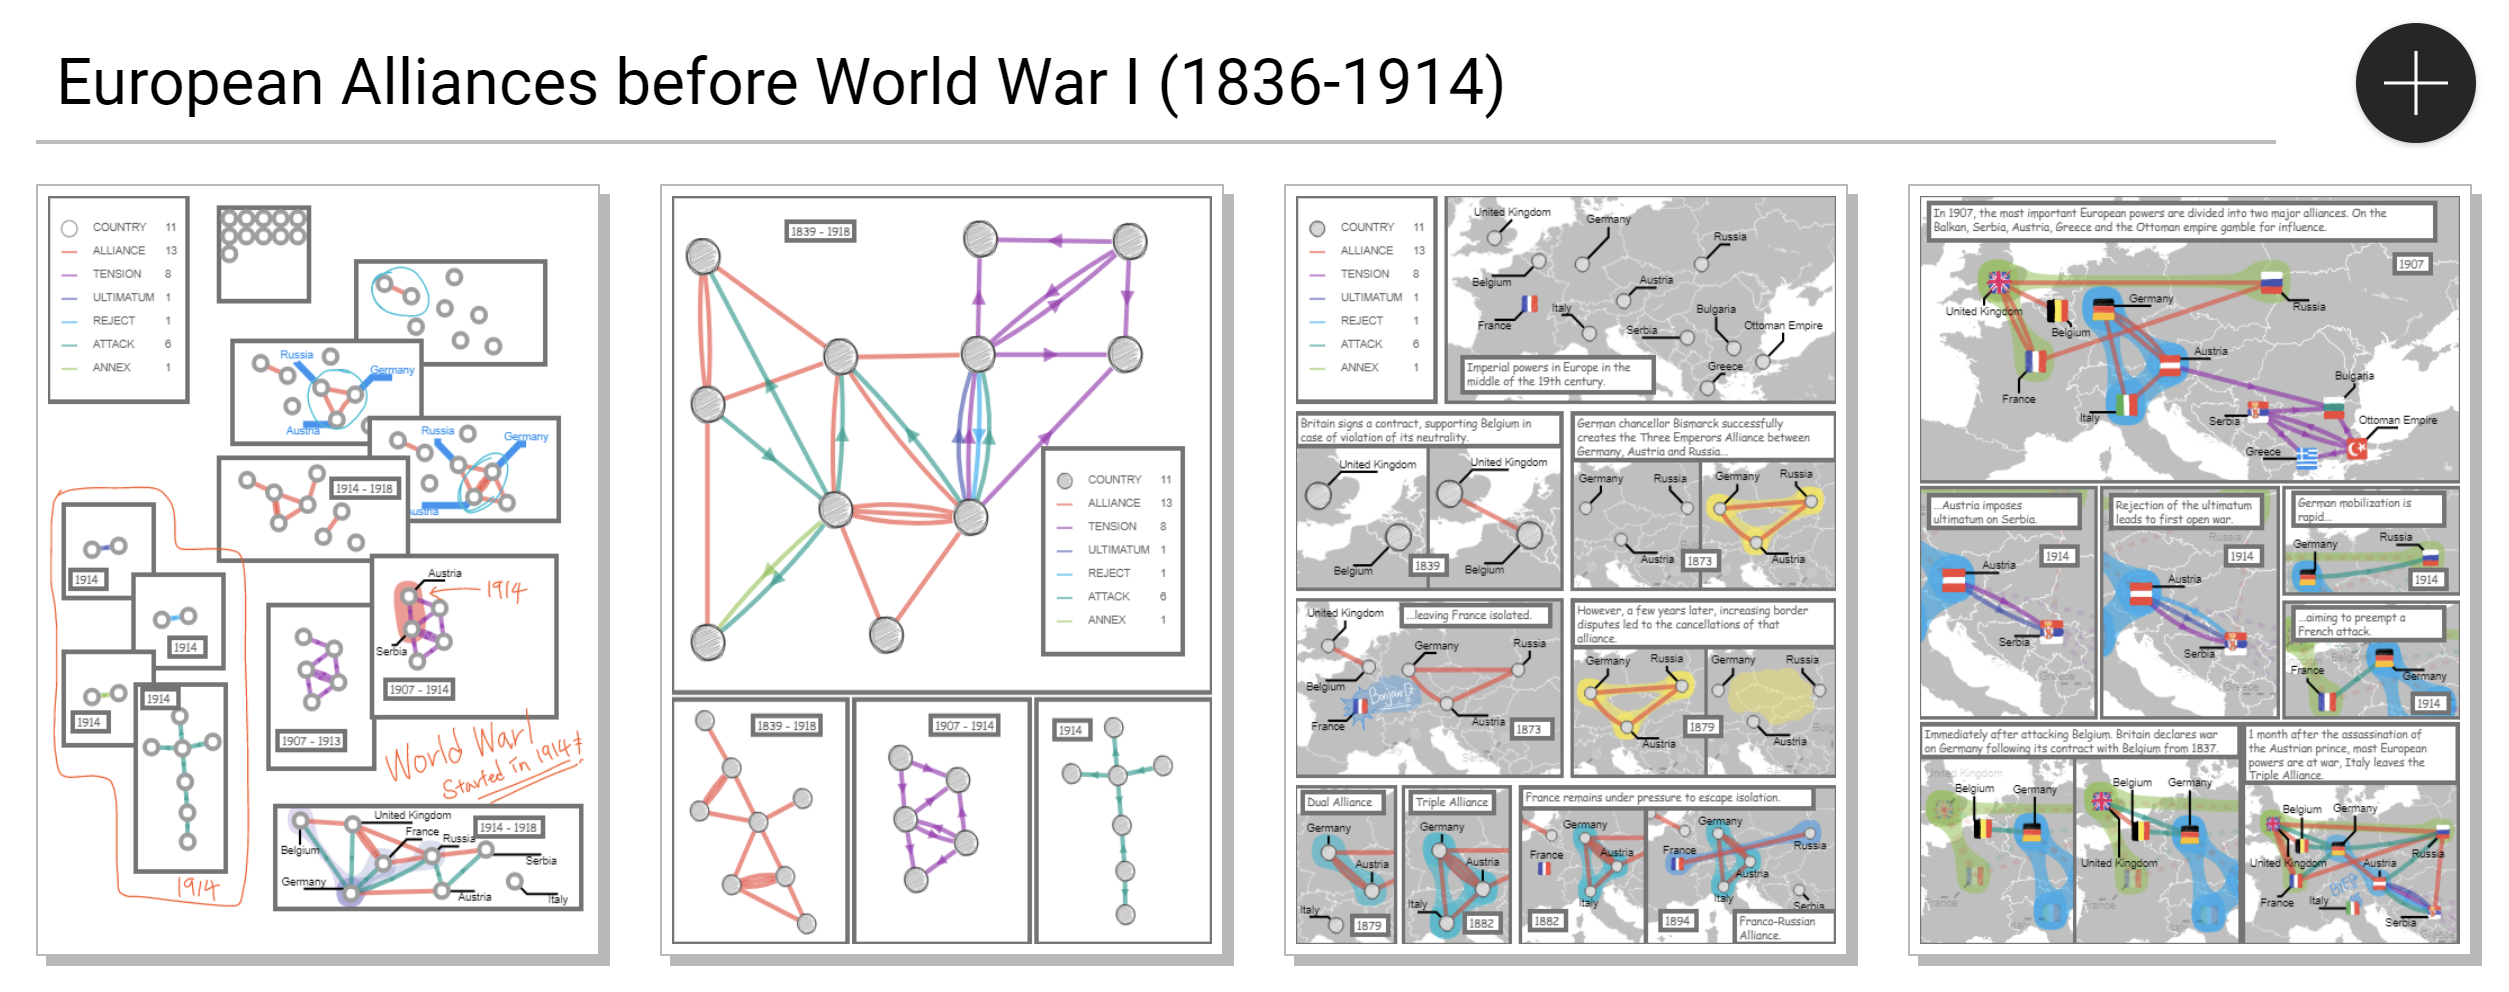
\includegraphics[width=\linewidth]{figures/comicbook} 
    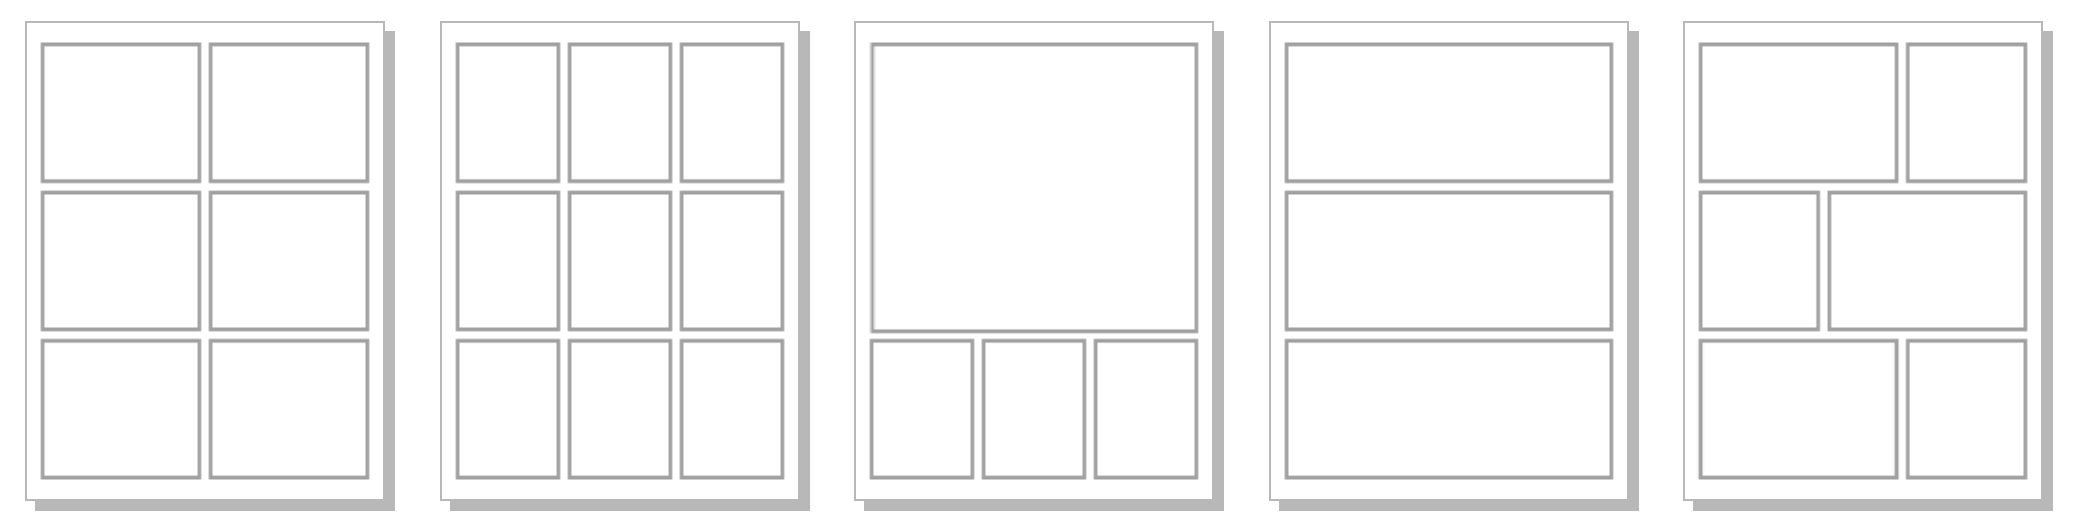
\includegraphics[width=1.0\columnwidth]{figures/layouts} 
    \caption{DataToon uses a comic book metaphor to allow authors to create multiple pages of data comics using more than one dataset. Each page can be created with a a predefined layout such as the ones shown in the second row.}
	\label{fig:comicbook}
     \vspace{-0.2cm}
\end{figure}


% Additional temporal filtering can be applied using the time slider that appears on demand when the author selects the panel (\autoref{fig:workflow}e).

% Dragging a node type onto the canvas creates a unit chart, while dragging a link type will create a node-link diagram. In a similar way, the user can progressively add more types to the existing panel to build a more complex visualization (e.g., a stacked unit chart with multiple groups of nodes and a node-link diagram with multiple groups of nodes and links). 

 

\bpstart{Acquiring different pen modes}
Content editing occurs through the use of the following pen modes:

\bstart{
\includegraphics[scale=0.03]{figures/draw_pen.png}  Pencil} mode is the default pen mode and allows for freeform inking on the canvas. If the author draws atop a content panel, the ink belongs to the panel and moves along with it when that content panel is manipulated. 

\bstart{
\includegraphics[scale=0.03]{figures/label_pen.png} Label} mode generates a text label for nodes and links and allows for adjusting label positions (\autoref{fig:teaser}F). Label and leader lines move when the element is moved.

\bstart{
\includegraphics[scale=0.03]{figures/highlight_pen.png}  Highlight} mode allows the author to lasso a set of nodes to highlight them in a colored group (\autoref{fig:teaser}F). As with labels, highlights also adjust when elements are moved.

\bstart{
\includegraphics[scale=0.03]{figures/filter_pen.png} Filter} mode allows the author to lasso a set of nodes to filter them from a panel or to create a new panel with these nodes (\autoref{fig:teaser}B). %\matt{Does one of these filter modes require pressing the pen button?}
Filtering can de-clutter panels and help focus on different subsets of the network. %\matt{violates ken's mantra}


\bstart{
\includegraphics[scale=0.03]{figures/layout_pen.png} Layout} mode leverages the high-precision of the digtial pen to adjust the positions of nodes and labels (\autoref{fig:interface}H). %\matt{also violates?} 
% The author can always resort to the automatic force-directed layout if necessary (\autoref{fig:interface}I). \matt{too much detail}

\bstart{
\includegraphics[scale=0.03]{figures/magic_pen.png} Magic} mode offers a way to automatically generate content panels (\autoref{fig:teaser}C, D), described in more detail below. 

\bstart{
\includegraphics[scale=0.03]{figures/eraser_pen.png} Eraser} mode deletes any item on the canvas including panels, ink, annotations, and highlights. This mode can also be invoked via the pen's eraser button, should it have one.  

\bstart{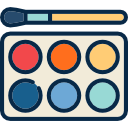
\includegraphics[scale=0.03]{figures/palette.png} Palette} mode allows the author to choose a different color, line thickness, and fill opacity, which will be applied to subsequent pencil strokes, annotations, and highlights.

% DataToon provides rich annotation and highlighting options by combining both freeform sketching and data-aware annotation (\textbf{C1}). Using the \textit{Annotation} pen, the author can lasso a set of nodes to show them in the foreground while muting the rest (\autoref{fig:workflow}f) or 

% generate a colored bubble surrounding them with the pen button pressed (\autoref{fig:workflow}h). The author can also create a node label by drawing a line out of each node (\autoref{fig:workflow}b). These types of annotations are all data-driven, making it easier to update iteratively. For instance, if the author updates the position of a node, the corresponding label and bubble are automatically updated. Just like the regular pencil, the author can choose a different style, and the selected style will then be applied to the style of the annotation. 

% \bpstart{Control 
\includegraphics[scale=0.05]{figures/control_pen.png}}
% To control which part of the content to show in the panel (e.g., cut-out or lens~\cite{bachdesign}), \toolname{} supports simple panning and zooming through the \textit{Control} pen (\autoref{fig:workflow}f). The author can also control the layout of a visualization (i.e., unit chart or node link diagram) that is initially auto-generated (\autoref{fig:workflow}b), as well as the positions of labels. 


% \bpstart{Transition 
\includegraphics[scale=0.05]{figures/transition_pen.png}}
% \toolname{} currently provides three automatic transitions, namely a temporal sequence, build-up of data dimensions, and zoom transform~\cite{bachdesign} (\autoref{fig:transitions}). To create the transitions, the author needs to draw a path from one panel to another using the \textit{Transition} pen. \toolname{} then tries to interpolate the two panels by detecting the difference between them. A typical continuous value interpolation works for the temporal sequencing and zoom transition (e.g., 2014 $\rightarrow$ \{2015,2016,2017\} $\rightarrow$ 2018). For the build-up transition, we progressively add or remove filters (i.e., node type or link type). The greater the distance between the panels is, the more transition panels are generated along the path.



% All the visual elements on the canvas can be directly manipulated through pen and multi-touch interaction. 
\vspace{2mm}
\bpstart{Drawing custom node and link representations}
% Finally,  author can update the visual encoding of the data dimension by tapping its current encoding in the legend panel .
A secondary canvas is invoked when the author taps on the iconic representation of a node or link type in the legend (\autoref{fig:interface}D). 
Within this canvas, the author can draw a new iconic representation for the selected node or link type, and this custom representation is immediately propagated across the comic for consistency (D2). 
% There are mainly two ways to modify the visual encoding, at the data point level and dimension level. When the author taps the visual encoding of a data dimension (node or link type) in the legend panel, it invokes the contextual canvas in which the author can draw a custom icon. 
The author can also invoke this canvas to change the representation of a single node or link, by tapping it with the pen while in pencil mode (
\includegraphics[scale=0.025]{figures/draw_pen.png}). 

 
%\begin{figure}[!t]
%    \centering
%    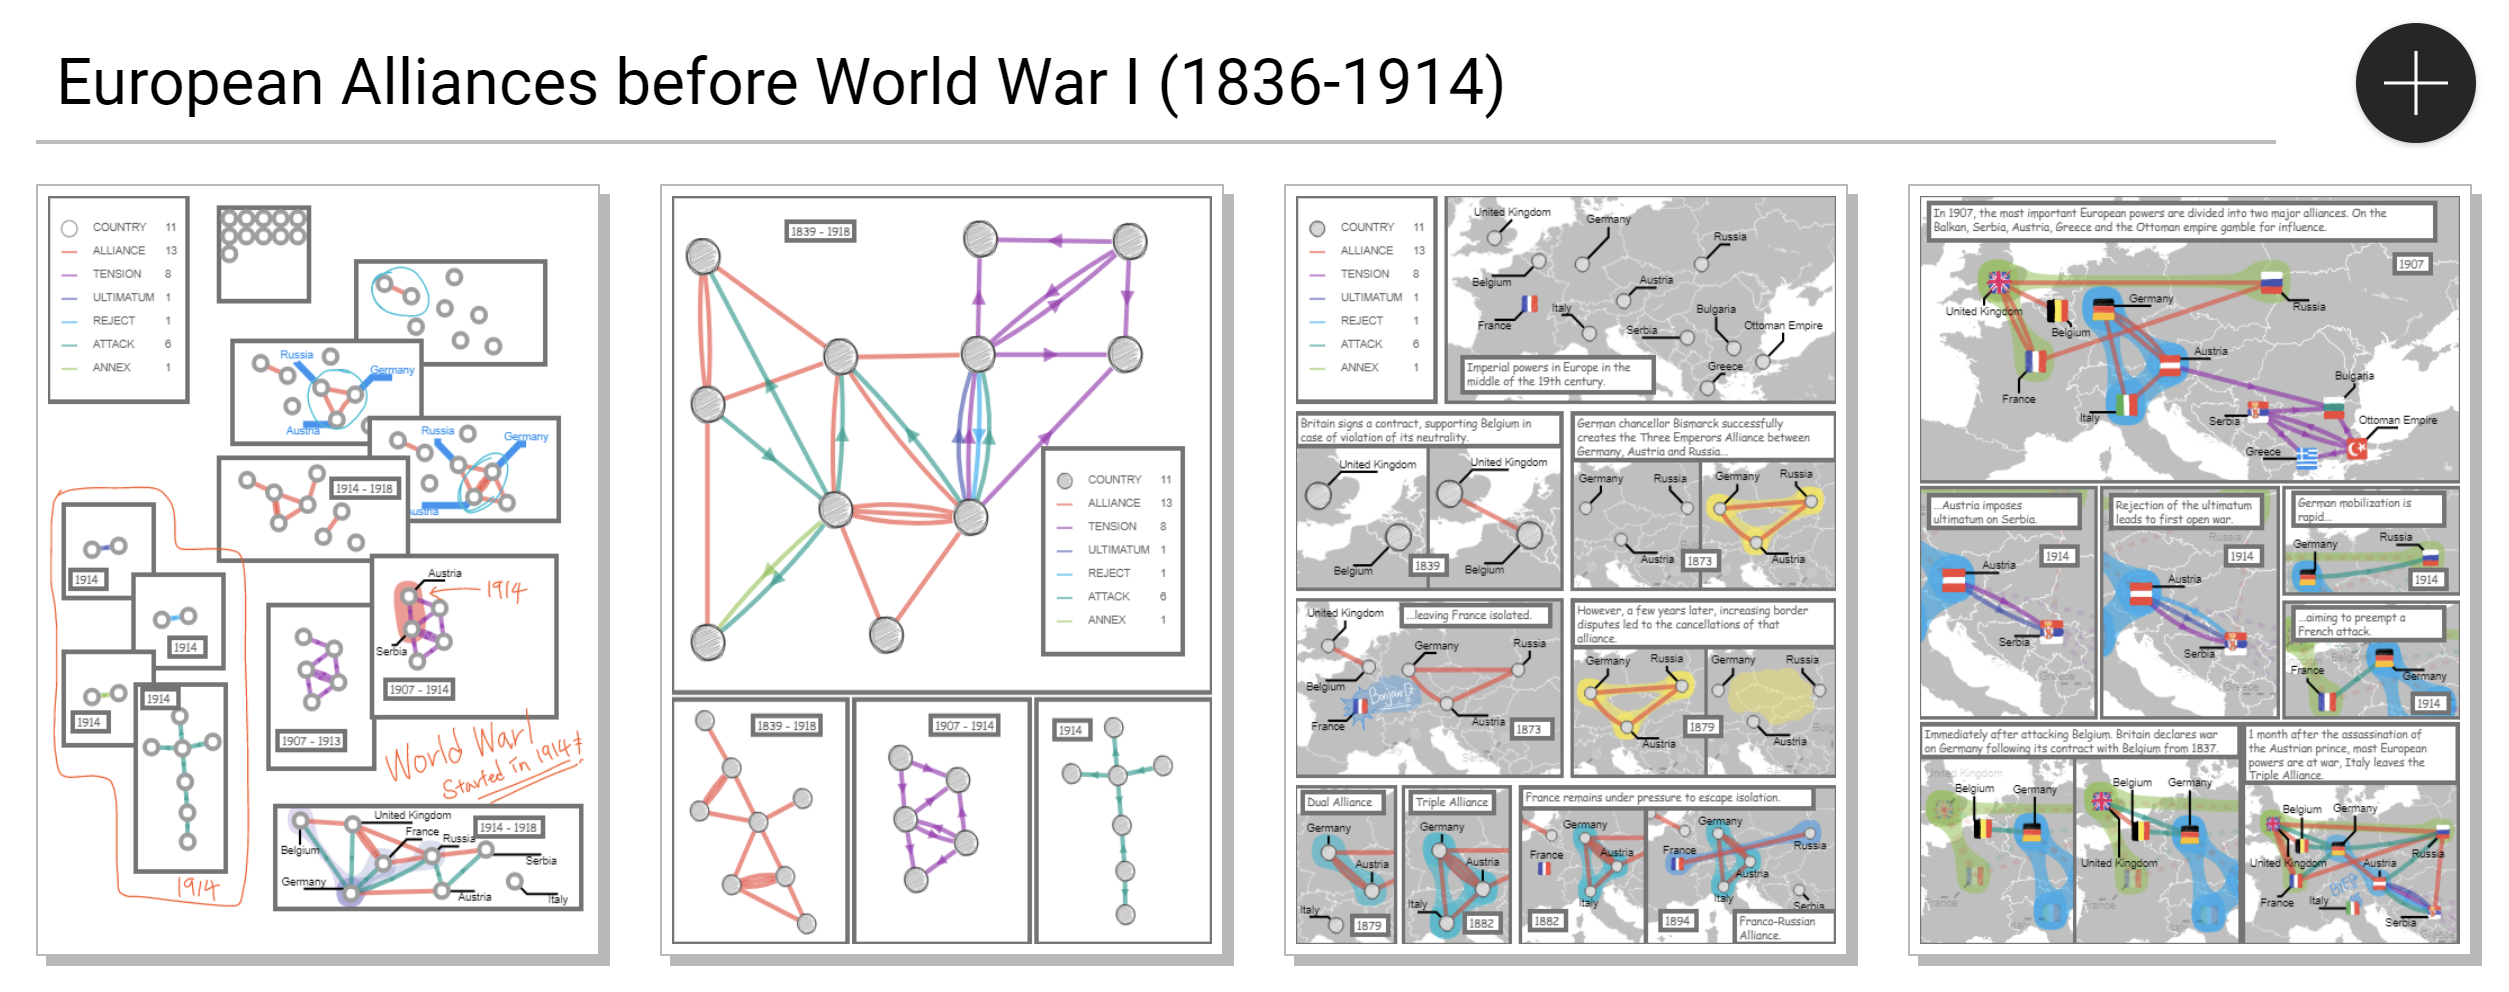
\includegraphics[width=\linewidth ]{figures/comicbook} 
%    \caption{DataToon uses a comic book metaphor to allow authors to create multiple pages of data comics using more than one dataset.}
%    \label{fig:comicbook}
%    \vspace{-0.2cm}
%\end{figure}
 
 

% \clearpage
% The reading order of the layout is assumed to follow the Z-path~\cite{cohn2014architecture}, guiding the reader from left to right, and then down). 
 

% A meaningful order and relation between a set of panels in comics can help creating a narrative [28]. A narrative can be linear, e.g., an explanation that spans over multiple panels, a sequence of question-and-answer, a temporal change, an exposé that contextualizes a dataset [11]. A narrative can further be non-linear [23, 36] or entirely open, inviting the reader to explore on their own, possibly after a guided introduction (martini-glass structure [48]). Our dimension of content relation describes how the panel content relates. Relations between just two panels have been described as transitions by McCloud [41] for traditional comics and include time steps (moment-to-moment), actions (action-to-action), characters or objects (subject-to-subject), places or scenes (scene-to-scene), aspects (aspect-to-aspect), or no specific relation at all (non-sequitur). Similar transitions have been described for data comics [10] and which reflect the more general taxonomy by Hullman et al. [33] on sequences in narrative visualizations: temporal, spatial, granular, comparison, causal, dialog. These transitions and categories have been inspirational to our dimension of content relation with some categories maintained: temporal, granular, facets.
% To alleviate the cost of generating intermediate panels

\begin{figure}[!tb]
    \centering
    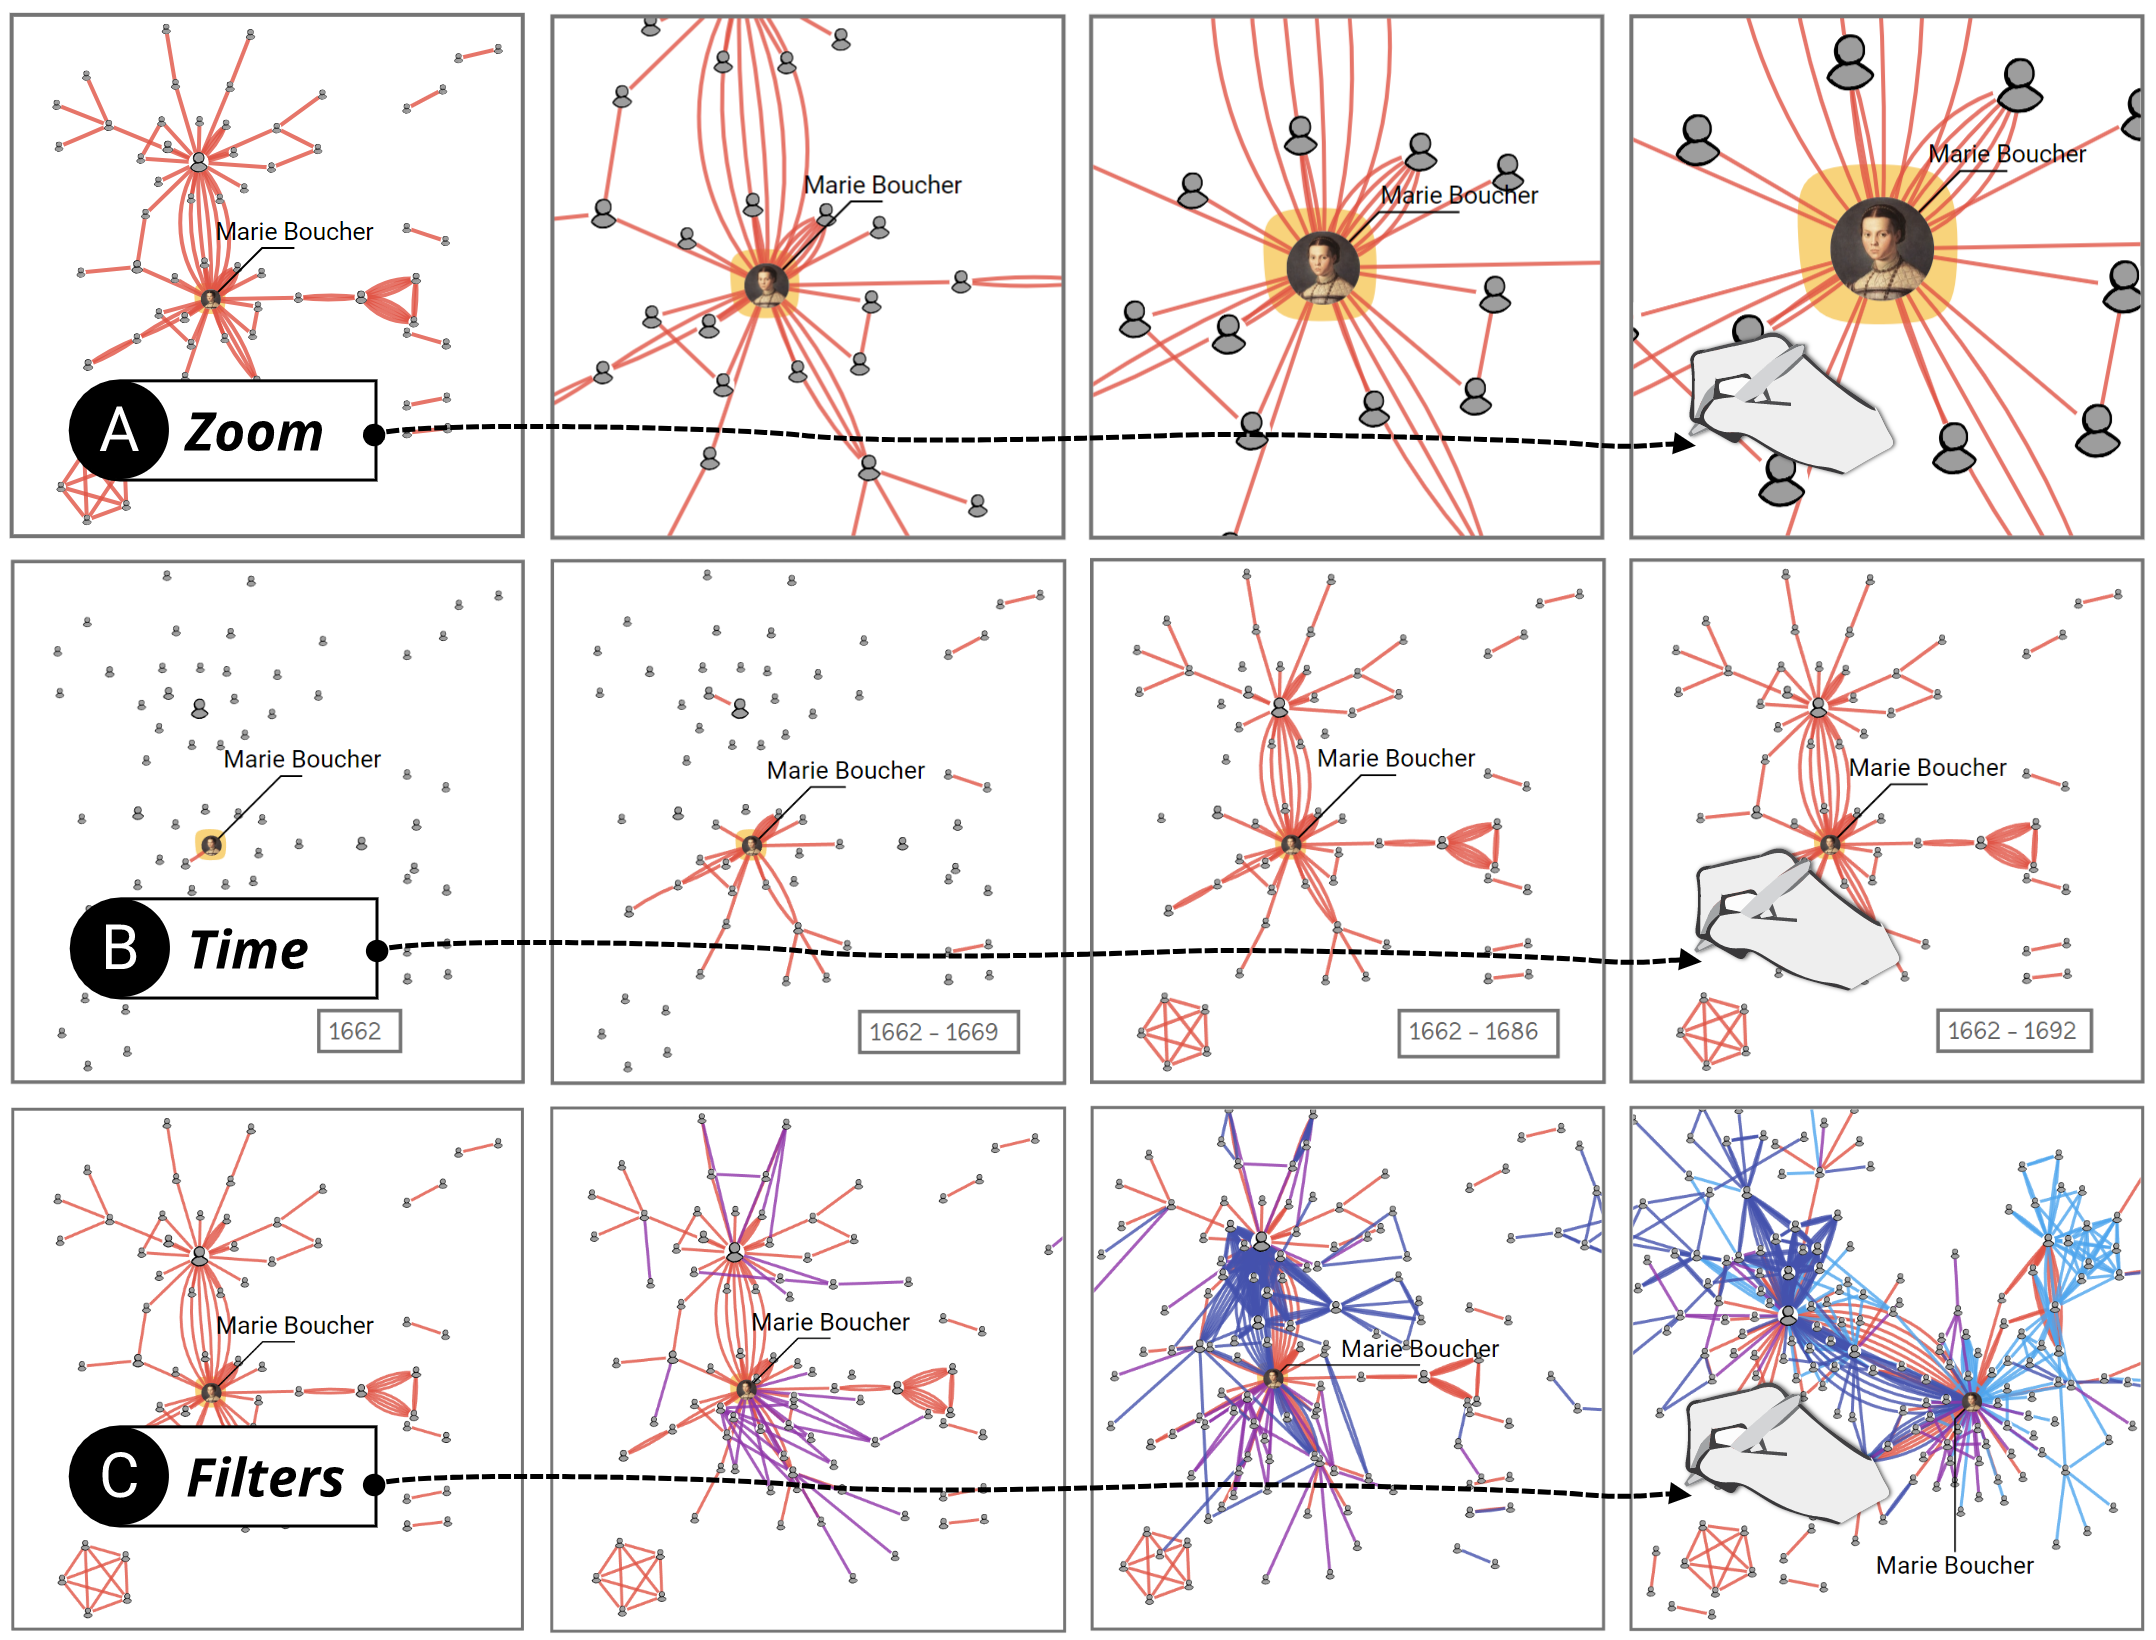
\includegraphics[width=\linewidth ]{figures/transition} 
     \vspace{-0.3cm}
    \caption{Automatic transitions between panels involve interpolating differences between panels, incorporating zoom levels, time ranges, filters, and combinations thereof.}
    \label{fig:transition}
    \vspace{-0.2cm}
\end{figure}

% \rev{geocoding if possibe}

 
 
%  as well as interactions of panel sizes. 

% Unlike a typical linear sequencing in other data storytelling tools, this can offer a nonlinear reading experience.


% panels contains a snapshot of data. scenes. time and location are 


% a visual data story consists of spatial juxtaposition of visualization panels and captions, data-driven and graphical annotations

% Panels as scenes. Each panel has data bindings determined through various filters. Pan and Zoom further defines the scene. 

% Sizing panels further allows manipulating the perception of the narrative. 
% Flow is established through the arragenment of panels. Narration is accomblished using the annotations. 

% non-linear structure
% We use space to convey both time and 

% a narrative flow
\vspace{-2mm}
\subsection{Facilitating Ideation}
\toolname{} provides several ways to scaffold and accelerate the data comics creation process (D1):

\bstart{1. Multiple pages and layout templates} facilitate the creation of multiple iterations of comics (\autoref{fig:comicbook}). Pages can load different datasets or contain different notes. Templates are a set of panel layouts commonly used in comics~\cite{bachdesign} such as grid, overview+detail, parallel, and staggered. 
When selected, the new page is auto-populated with empty content panels specified by the template. Authors can simply drag data on top of them to fill them.
% with panels based on the layout. They currently do not fill the content of the panels but are designed to scaffold a narrative structure. We leave automatically filling the content of the layout as future work. 

\bstart{2. Automatic transitions.}
% to get recommendations for next panels or between two panels to create transitions. 
\toolname{} creates intermediary panels by interpolating the difference between the two panels, taking into account their respective panel sizes, data filters, and zoom states (\autoref{fig:transition}). 
%\matt{Re: R1's review, What happens to backroung images?}
These transitions may also incorporate a temporal progression between two time filter states and the addition or removal of nodes and links~\cite{bachdesign}. 
It does not, however, attempt to interpolate annotations between two panels.

As an example, if a source panel and a target panel have zoom factors of 1.0 and 1.8 respectively, intermediary panels will have interpolated zoom factors between 1.0 and 1.8. In addition, if the source and target panels have different sizes and display data at different time periods, \toolname{} will interpolate over these dimensions as well, producing intermediary panels that would gradually increase in size and depict a progression over time intervals.  
%Similarly, \toolname{} applies a continuous value interpolation for panel size transformations and temporal sequence shifts (e.g., 1873 $\rightarrow$ [1885,1897] $\rightarrow$ 1914), progressively adding or removing nodes and links (e.g., {\textit{Alliance}, \textit{Tension}} $\rightarrow$ [ {\textit{Alliance}}, {\textit{Alliance}, \textit{Ultimatum}} ] $\rightarrow$ {\textit{Alliance}, \textit{Ultimatum}, \textit{Reject}}).

\toolname{} places intermediary panels along the path drawn by the author. Greater distances between panels results in more intermediary panels along the path. It discretizes the path and conducts a linear search for panel positions, while ensuring no overlap between intermediary panels. 

\vspace{2mm}
\bstart{3. Panel suggestions}
% To suggest next panels from one panel, it relies on detecting sub-network patterns in the panel data (\autoref{fig:suggestion}). 
 for new panels are shown in two contexts: either when loading a new dataset or when drawing a line out of a panel using the Magic pen. 
In the first case, it attempts to detect interesting subnetwork patterns in the whole dataset and places suggested panels at the left side of the canvas. 
This helps authors become familiar with the dataset and serves to kickstart the story design process. 
In the second case, it takes into account the current state of the panel and detects patterns within the panel to generate suggestions. 
It thereby enables authors to discover potential compelling directions for their story. Similar to transitions, these suggested panels are placed along the path the author draws, while preventing overlap between them. 

To detect patterns in the network data, \toolname{} relies on a pattern detection engine. The engine accepts any network data including highlighted nodes as input and returns a list of detected patterns. It currently looks for four structural patterns including articulation points (or bridges), cliques, hubs, and communities (\autoref{fig:suggestion}). Once patterns are found, it heuristically prunes the results such as by removing overlapping patterns (e.g., a bridge and a hub can often show a completely identical structure), as well as cliques with less than four nodes. Finally, it ranks the patterns based on how much each pattern overlaps with the source data. This is to promote closure between the source panel and the suggested panel. Finally, the rankings give a high priority to patterns that contain highlighted nodes (\autoref{fig:suggestion} C).

\begin{figure}[!tb]
    \centering
    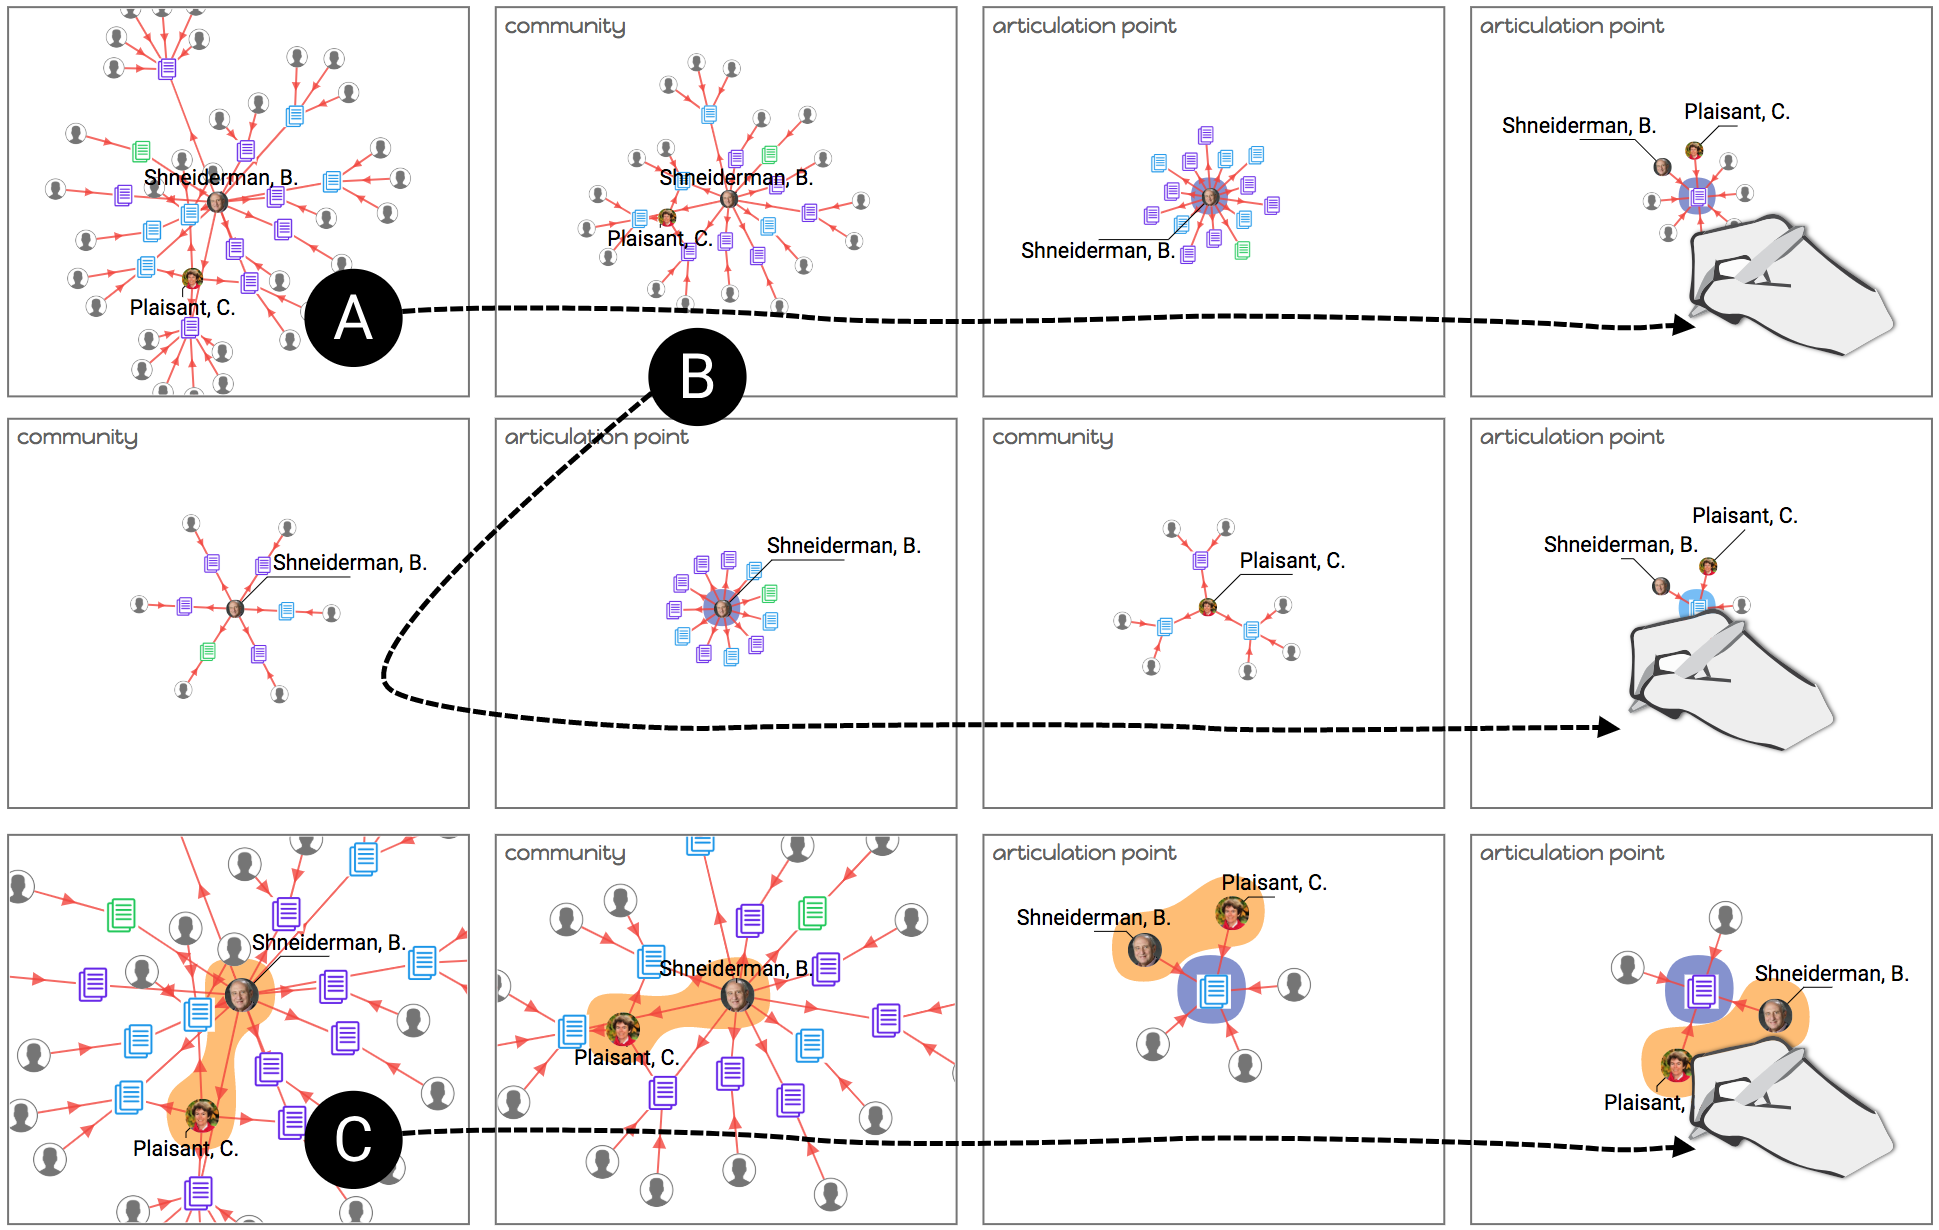
\includegraphics[width=\linewidth ]{figures/suggestion.png} 
    % \vspace{-0.3cm}
    \caption{Automatic panel suggestions depicts structural patterns: communities, hubs, articulation points, and cliques. The author can trigger suggestions from existing panels (A) and suggested panels (B). Patterns are ranked based on network coverage and inclusion of highlighted nodes (C).}
    \label{fig:suggestion}
\vspace{-0.5cm}
\end{figure}

\subsection{Implementation Details}
\toolname{} is a browser-based application written in Javascript. It uses React.js for building user interface components and Redux.js for application state management. It uses WebCoLa
~\cite{webcola} to generate the layout of the node-link diagram and a Javascript implementation~\cite{bubblesets} of Bubble Sets~\cite{collins2009bubble} to highlight a group of nodes as a cluster. \toolname{} consists of a front-end interface without a back-end server, though one can be attached if needed; currently, \toolname{} makes use of localStorage and indexedDB in HTML5 to persist the application state. The panel recommendation engine is implemented in Python and uses NetworkX to detect patterns~\cite{networkx}. 

% We also make use of utility functions in D3~\cite{d3} such as pan and zoom, and react-annotation for labelling~\cite{annotation}. 


% and available on GitHub (\rev{https://github.com/nathalieriche/datacomics/})